
\documentclass[journal,12pt,twocolumn]{IEEEtran}
\usepackage{graphicx}
\graphicspath{{./figs/}}{}
\usepackage{amsmath,amssymb,amsfonts}
\usepackage{gensymb}
\usepackage{stackengine}
\usepackage{scalerel}
\newcommand{\myvec}[1]{\ensuremath{\begin{pmatrix}#1\end{pmatrix}}}

\let\vec\mathbf

\newlength\triwidth
\newcommand\tridelt[1]{%
  \setlength\triwidth{\widthof{#1\ }}%
  \stackengine{-.1\triwidth}{#1\ }%
    {\scaleto{\Delta}{1\triwidth}}{O}{c}{F}{F}{L}%
}
\title{
Matrix-circle
}
\author{Kukunuri Sampath Govardhan}
\begin{document}
\maketitle
\tableofcontents
\section{Problem Statement}
\begin{flushleft}
    If circles x$^2$+y$^2$+2x+2ky+6 = 0,  x$^2$+y$^2$+2ky+k = 0\\
intersect orthogonally then find k.\\
\end{flushleft}
\section{Construction}
\begin{figure}[h]
    \centering
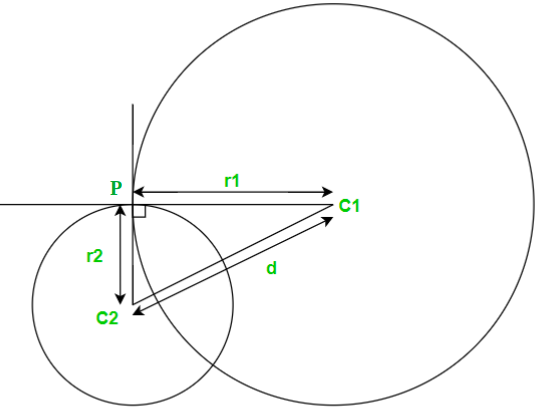
\includegraphics[width=\columnwidth]{figs/Assignment5.png}
    \caption{Orthogonal Circles}
    \label{fig:my_label}
\end{figure}
\vspace{2cm}
\begin{table}[h]
    \centering
    \begin{tabular}{|c|c|c|}
       \hline
       \textbf{Symbol}&\textbf{Value}&\textbf{Description}  \\
       \hline
        $\vec{C1}$ & $\begin{pmatrix}
  -1\\
  -k\\
 \end{pmatrix}$% 
 & Center of circle C1\\
        \hline
        $\vec{C2}$ & $\begin{pmatrix}
  0\\
  -k\\
 \end{pmatrix}$% 
 & Center of circle C2\\
        \hline
        $\vec{P}$ &  $\vec{X}$ & Radius of circle C1 \\
        \hline
        $\theta$ & 90\textdegree & Given that C1 and C2 are Orthogonal\\
        \hline
        d & 1 & Distance between centers of the circles\\
        \hline
    \end{tabular}
    \caption{Parameters}
    \label{tab:my_label}
\end{table}
\vspace{3cm}
Standard form of a circle in matrix form is \\
\begin{center}
    $\vec{xVx^T} + 2\vec{u^Tx}$ + f = 0 \\
\end{center}
where, $$\vec{V} = \myvec{ 1 & 0 \\ 0 & 1}, Center \vec{C} = -\vec{V^{-1}u^T},$$
\begin{center}
Radius of a circle is r = $\sqrt{\vec{u^T}\vec{u}-f}$
\end{center}
Equation of given circles can be represented in matrix form as\\
\begin{equation}
    \vec{xx^T} + 2\myvec{ 1 & k}\vec{x} + 6 = 0 \label{eq-1}
\end{equation}
\begin{equation}
    \vec{xx^T} + 2\myvec{ 0 & k}\vec{x} + k = 0 \label{eq-2}
\end{equation}

where,\\
$$\vec{u_1} = \myvec{ 1 \\ k}, \vec{u_2} = \myvec{ 0 \\ k}, f_1 = 6 , f_2 = k$$
$$\vec{C_1} = \myvec{-1 & -k}, \vec{C_2} = \myvec{0 & -k}$$\\
\\
The radius of first circle is  $r_1$ = $\sqrt{k^2 -5}$\\
\\
The radius of Second Circle is $r_2$ = $\sqrt{k^2 -k}$\\

Given that, the circles are orthogonal so the angle between the radii r1 and r2 is 90\textdegree.  \\
\\
From figure \tridelt.PC1C2 is a Right angled triangle with hypotenuse d = $||C1-C2||$ .  \\
\\
So, by using \textbf{Pythagoraus theorem}  \\
\\
\begin{equation}
    \vec{||C_1 - C_2||^2 = ||C_1 - P||^2+||C_2 - P||^2}
\end{equation}
\\
Therefore,$$\vec{||C_1 - C_2||^2 = r_1^2+r_2^2}$$
\begin{equation}
    1 = k^2 -5 + k^2 - k
\end{equation}
Yielding, k = 2 or -$\frac{3}{2}$ \\
Therefore, the value of k is \\
\begin{center}
    \textbf{k = 2} or -$\boldsymbol{\frac{3}{2}}$\\
\end{center}
\end{document}
